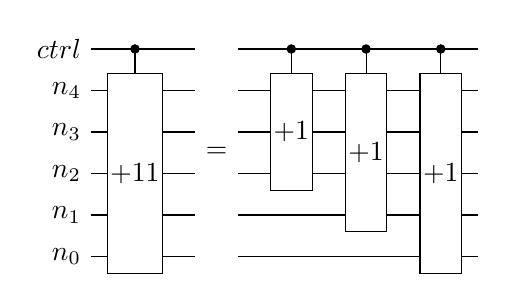
\begin{tikzpicture}[scale=1.000000,x=1pt,y=1pt]
\filldraw[color=white] (0.000000, -7.500000) rectangle (140.000000, 82.500000);
% Drawing wires
% Line 1: ctrl W ctrl
\draw[color=black] (0.000000,75.000000) -- (140.000000,75.000000);
\draw[color=black] (0.000000,75.000000) node[left] {$ctrl$};
% Line 2: n4 W n_4
\draw[color=black] (0.000000,60.000000) -- (140.000000,60.000000);
\draw[color=black] (0.000000,60.000000) node[left] {$n_4$};
% Line 3: n3 W n_3
\draw[color=black] (0.000000,45.000000) -- (140.000000,45.000000);
\draw[color=black] (0.000000,45.000000) node[left] {$n_3$};
% Line 4: n2 W n_2
\draw[color=black] (0.000000,30.000000) -- (140.000000,30.000000);
\draw[color=black] (0.000000,30.000000) node[left] {$n_2$};
% Line 5: n1 W n_1
\draw[color=black] (0.000000,15.000000) -- (140.000000,15.000000);
\draw[color=black] (0.000000,15.000000) node[left] {$n_1$};
% Line 6: n0 W n_0
\draw[color=black] (0.000000,0.000000) -- (140.000000,0.000000);
\draw[color=black] (0.000000,0.000000) node[left] {$n_0$};
% Done with wires; drawing gates
% Line 8: n4 n3 n2 n1 n0 G width=20 $+11$ ctrl
\draw (16.000000,75.000000) -- (16.000000,0.000000);
\begin{scope}
\draw[fill=white] (16.000000, 30.000000) +(-45.000000:14.142136pt and 50.911688pt) -- +(45.000000:14.142136pt and 50.911688pt) -- +(135.000000:14.142136pt and 50.911688pt) -- +(225.000000:14.142136pt and 50.911688pt) -- cycle;
\clip (16.000000, 30.000000) +(-45.000000:14.142136pt and 50.911688pt) -- +(45.000000:14.142136pt and 50.911688pt) -- +(135.000000:14.142136pt and 50.911688pt) -- +(225.000000:14.142136pt and 50.911688pt) -- cycle;
\draw (16.000000, 30.000000) node {$+11$};
\end{scope}
\filldraw (16.000000, 75.000000) circle(1.500000pt);
% Line 10: =
\draw[fill=white,color=white] (38.000000, -6.000000) rectangle (53.000000, 81.000000);
\draw (45.500000, 37.500000) node {$=$};
% Line 12: n4 n3 n2 G width=15 $+1$ ctrl
\draw (72.500000,75.000000) -- (72.500000,30.000000);
\begin{scope}
\draw[fill=white] (72.500000, 45.000000) +(-45.000000:10.606602pt and 29.698485pt) -- +(45.000000:10.606602pt and 29.698485pt) -- +(135.000000:10.606602pt and 29.698485pt) -- +(225.000000:10.606602pt and 29.698485pt) -- cycle;
\clip (72.500000, 45.000000) +(-45.000000:10.606602pt and 29.698485pt) -- +(45.000000:10.606602pt and 29.698485pt) -- +(135.000000:10.606602pt and 29.698485pt) -- +(225.000000:10.606602pt and 29.698485pt) -- cycle;
\draw (72.500000, 45.000000) node {$+1$};
\end{scope}
\filldraw (72.500000, 75.000000) circle(1.500000pt);
% Line 13: n4 n3 n2 n1 G width=15 $+1$ ctrl
\draw (99.500000,75.000000) -- (99.500000,15.000000);
\begin{scope}
\draw[fill=white] (99.500000, 37.500000) +(-45.000000:10.606602pt and 40.305087pt) -- +(45.000000:10.606602pt and 40.305087pt) -- +(135.000000:10.606602pt and 40.305087pt) -- +(225.000000:10.606602pt and 40.305087pt) -- cycle;
\clip (99.500000, 37.500000) +(-45.000000:10.606602pt and 40.305087pt) -- +(45.000000:10.606602pt and 40.305087pt) -- +(135.000000:10.606602pt and 40.305087pt) -- +(225.000000:10.606602pt and 40.305087pt) -- cycle;
\draw (99.500000, 37.500000) node {$+1$};
\end{scope}
\filldraw (99.500000, 75.000000) circle(1.500000pt);
% Line 14: n4 n3 n2 n1 n0 G width=15 $+1$ ctrl
\draw (126.500000,75.000000) -- (126.500000,0.000000);
\begin{scope}
\draw[fill=white] (126.500000, 30.000000) +(-45.000000:10.606602pt and 50.911688pt) -- +(45.000000:10.606602pt and 50.911688pt) -- +(135.000000:10.606602pt and 50.911688pt) -- +(225.000000:10.606602pt and 50.911688pt) -- cycle;
\clip (126.500000, 30.000000) +(-45.000000:10.606602pt and 50.911688pt) -- +(45.000000:10.606602pt and 50.911688pt) -- +(135.000000:10.606602pt and 50.911688pt) -- +(225.000000:10.606602pt and 50.911688pt) -- cycle;
\draw (126.500000, 30.000000) node {$+1$};
\end{scope}
\filldraw (126.500000, 75.000000) circle(1.500000pt);
% Done with gates; drawing ending labels
% Done with ending labels; drawing cut lines and comments
% Done with comments
\end{tikzpicture}
